\documentclass[onecolumn, draftclsnofoot,10pt, compsoc]{IEEEtran}
\usepackage{graphicx}
\usepackage{url}
\usepackage{svg}
\usepackage{setspace}
\usepackage{float}
\usepackage{longtable}
\usepackage{pgfgantt}
\usepackage{amsmath}
\usepackage{amssymb}
%\usepackage{minted}
\usepackage{geometry}
\geometry{textheight=9.5in, textwidth=7in}


\def \subparagraph {.}

\usepackage{titlesec}
\usepackage{hyperref}

\titleclass{\threesection}{straight}[\subsection]
\titleclass{\foursection}{straight}[\subsection]


\newcounter{threesection}[subsubsection]
\newcounter{foursection}[threesection]

\renewcommand\thethreesection{\thesubsubsection.\arabic{threesection}}
\renewcommand\thefoursection{\thethreesection.\arabic{foursection}}

\renewcommand\theparagraph{\thethreesection.\arabic{paragraph}}
\renewcommand\theparagraph{\thefoursection.\arabic{paragraph}}

\titleformat{\threesection}
  {\normalfont\normalsize\bfseries}{\thethreesection}{1em}{}
\titlespacing*{\threesection}
{0pt}{3.25ex plus 1ex minus .2ex}{1.5ex plus .2ex}

\titleformat{\foursection}
  {\normalfont\normalsize\bfseries}{\thefoursection}{1em}{}
\titlespacing*{\foursection}
{0pt}{3.25ex plus 1ex minus .2ex}{1.5ex plus .2ex}


\makeatletter
\renewcommand\paragraph{\@startsection{paragraph}{6}{\z@}%
  {3.25ex \@plus1ex \@minus.2ex}%
  {-1em}%
  {\normalfont\normalsize\bfseries}}
\renewcommand\subparagraph{\@startsection{subparagraph}{7}{\parindent}%
  {3.25ex \@plus1ex \@minus .2ex}%
  {-1em}%
  {\normalfont\normalsize\bfseries}}
\def\toclevel@threesection{4}
\def\toclevel@foursection{5}
\def\toclevel@paragraph{6}
\def\toclevel@paragraph{7}
\def\l@threesection{\@dottedtocline{4}{7em}{4em}}
\def\l@foursection{\@dottedtocline{5}{10em}{5em}}
\def\l@paragraph{\@dottedtocline{6}{14em}{6em}}
\def\l@subparagraph{\@dottedtocline{7}{19em}{7em}}
\makeatother

\setcounter{secnumdepth}{4}
\setcounter{tocdepth}{4}
\setcounter{secnumdepth}{5}
\setcounter{tocdepth}{5}


% 1. Fill in these details
\def \CapstoneTeamName{			PolyVox}
\def \CapstoneTeamNumber{		66}
\def \GroupMemberOne{			Chris Bakkom}
\def \GroupMemberTwo{			Richard Cunard}
\def \GroupMemberThree{			Braxton Cuneo}
\def \CapstoneProjectName{		3D Virtual Reality Painting}
\def \CapstoneSponsorCompany{		EECS}
\def \CapstoneSponsorPersonOne{		Dr. Kirsten Winters}
\def \CapstoneSponsorPersonTwo{		Dr. Mike Bailey}
\def \CapstoneSponsorPersonTwo{		Dr. Mike Bailey}

% 2. Uncomment the appropriate line below so that the document type works
\def \DocType{		%Problem Statement
				%Requirements Document
				%Technology Review
				%Software Design Description (Draft 1/5/2018)
				
				Spring Midterm Progress Report
				}
			
\newcommand{\NameSigPair}[1]{\par
\makebox[2.75in][r]{#1} \hfil 	\makebox[3.25in]{\makebox[2.25in]{\hrulefill} \hfill		\makebox[.75in]{\hrulefill}}
\par\vspace{-12pt} \textit{\tiny\noindent
\makebox[2.75in]{} \hfil		\makebox[3.25in]{\makebox[2.25in][r]{Signature} \hfill	\makebox[.75in][r]{Date}}}}
% 3. If the document is not to be signed, uncomment the RENEWcommand below
%\renewcommand{\NameSigPair}[1]{#1}

%%%%%%%%%%%%%%%%%%%%%%%%%%%%%%%%%%%%%%%
\begin{document}
\begin{titlepage}
    \pagenumbering{gobble}
    \begin{singlespace}
    	\includegraphics[height=4cm]{coe_v_spot1}
        \hfill 
        % 4. If you have a logo, use this includegraphics command to put it on the coversheet.
        %\includegraphics[height=4cm]{CompanyLogo}   
        \par\vspace{.2in}
        \centering
        \scshape{
            \huge CS Capstone \DocType \par
            {\large\today}\par
            \vspace{.5in}
            \textbf{\Huge\CapstoneProjectName}\par
            \vfill
            {\large Prepared for}\par
            \Huge \CapstoneSponsorCompany\par
            \vspace{5pt}
            {\Large\NameSigPair{\CapstoneSponsorPersonOne}\par}
	    {\Large\NameSigPair{\CapstoneSponsorPersonTwo}\par}
            {\large Prepared by }\par
            Group\CapstoneTeamNumber\par
            % 5. comment out the line below this one if you do not wish to name your team
            \CapstoneTeamName\par 
            \vspace{5pt}
            {\Large
                \NameSigPair{\GroupMemberOne}\par
                \NameSigPair{\GroupMemberTwo}\par
                \NameSigPair{\GroupMemberThree}\par
            }
            \vspace{20pt}
        }
        \begin{abstract}
        % 6. Fill in your abstract
        Since the beginning of spring term, several features have been added to PolyVox and several aspects of PolyVox's old features have been optimized or otherwise improved. This includes the addition of diegetic interfaces for brush color, transparency, and scale selection as well as runtime and memory improvements for the back end. With these additions made, the PolyVox team plans to add a few final touches and polish pre-existing features in preparation for expo.
        
        \end{abstract}     
    \end{singlespace}
\end{titlepage}
\newpage
\pagenumbering{arabic}
\tableofcontents
% 7. uncomment this (if applicable). Consider adding a page break.
%\listoffigures
%\listoftables
\clearpage

% 8. now you write!

\subsection{References}
\bibliographystyle{IEEEtran}
\bibliography{Bibliography}{}

\section{Introduction}

\subsection{Goal of the project}
The initial concept of this project was to develop a VR-based 3D art program that employs the use of motion controls in order to allow a user to ‘paint’ in 3D space. From this description, the PolyVox team decided on a set of specific requirements for the program that would eventually come to be known as PolyVox. The system would be voxel based, in order to take advantage of the more efficient data manipulation that doing so would afford. The system would allow a user to create, modify and destroy 3D geometry. Additionally, the user would be able to scale the virtual scene, be able to save or load a given configuration of geometry (that is, a piece of artwork or a ‘scene’) from memory. Furthermore, all of the above mentioned features would be performed using motion controls associated with a virtual reality HMD. 

\subsection{Status of the project at the start of the term}
The system has been capable of the above requirements since the beginning of the term, when the first beta build was completed. The team's efforts this term have primarily been to expose these different features as a unified interface, improve the performance of existing features, and finish development of stretch goals if time permitted. The system now has a diegetic user interface that allows the user to operate the program via Oculus motion controls. The UI allows the user to control brush color, opacity, and save/load functionality. Additionally, the user can change the size and shape of their ‘brush’ object, as well as erase existing geometry using the motion controllers.

\subsection{Primary updates made to the program}
The updates made to the front and middle ends of the program primarily involve the connection or improvement of existing systems into the program. Updates to the back-end of the program have mainly been performance-focused. As stated above, the user interface now operates many of the program’s features. This includes a color picker screen which displays, in a two dimensional graph, the saturation and value, on which the user controls a cursor. This color picker also has two sliders, which control hue and opacity, and a save/load menu, through which a user can select either operation, causing a VR keyboard to appear before the user, allowing them to enter the name of the file they are saving or loading. Additionally, several updates to the graphics engine have been made, which have significantly improved general performance, with increases made to framerate, voxel resolution, and the ability to render transparent objects. 

\subsection{What is left to do}
With the engineering expo approaching, our team is primarily focused on finishing implementation of features and solidifying performance. The team intends to implement a ‘cursor’, which will provide a display of the current size, shape, and color their brush is set to. This will allow a user to more clearly determine what they will be creating when they use their ‘brush’. The team also experimenting with different UI configurations, such as following the user’s head movement or controller movement. Finally, the team needs to begin performing UI and stress tests to confirm that the program runs smoothly once converted into an executable.


\section{Chris Bakkom}



\subsection{Turning the UI from a non-diegetic to a diegetic one}
When the initial UI was designed, it was structured under a standard platform. This was a flat interface to add menu controls and function selection. This was set up as most normal menus are, in a 2D structure that is projected onto the 3D world. This would have been something that the user could pull up with a button press and then navigate with the buttons and analog stick on the VR controllers. This was sufficient in fulfilling the criteria for the project goals, but had a few problems.

This user interface was not only suboptimal for the environment it was projected on, it was also not comfortable for a VR user. By projecting a 2D screen onto the VR headset, this essentially redirected the flow of the environment. A user would find themselves using the application and become comfortable to objects existing in the same space as them. By introducing a UI that was static and disconnected with the rest of the scene, the interface was completely inconsistent to user expectations. This made the program menu uncomfortable and hard to use. 

This is was pushed the decision to make the UI a diegetic one. This means that the user interface would be a rendered 3D object that exists in the environment instead of placed on top of the screen. Initially this was set to a camera render section that interpolated the 2D position into a 3D one. However, this was taking too much processing time to layer each UI element and compare it to the rest of the scene. Instead the UI was adapted so that each element would be rendered in world space. All of the UI was restructured in its parent hierarchy to follow this structure. This was much more natural solution to VR user interfaces than the typical menu system. 

\subsection{Creating targeting rays for UI section}
When changing all the UI elements into world space objects, there was also the question of selection in 3-space. Often it was not intuitive to have buttons on the controllers do certain actions. Some of the things in the menu system worked for this, like color and brush selection. This is because users wanted to be able to change the color and brush style while they were painting. This required that some of the functions still be mapped to a controller input. However some elements of the UI, like sliders, buttons, and input fields still needed a way to be selectable in the 3D environment. 

From this issue came the implementation of the UI rays for menu selection. These are rays that are cast out from the VR controller so the user can activate certain items. Much like a mouse, the rays offers a point and click functionality. The user is now able to aim the ray with their VR controller at a UI element and use the trigger to “click” on one of the menu items. This allowed the world space menu to be accessible through more than just button presses and analog tilts. This allowed for the implementation of standard UI controls without managing their compatability with VR controls. 

\subsection{Head or hand tracked UI}
One of the design choices that still needs to be addressed is whether the UI should be tracked onto the head or hand of the user. When creating a UI that exists in the same 3D world as the user, there needs to be a pivot in which the UI is anchored to. This will allow the user to access the UI and make sure that it is not in the way of their work, while keeping its properties. The two ways proposed to make this happen is to anchor the UI onto the display itself or onto the one of the controllers.

If the UI is anchored to the head set then it can be accessed more easily, but may be prone to obscuring the viewport. While the anchor is attached to main view port, the user can easily turn their head toward one direction and find the functions they are looking for. This even cuts down on the number of controllers needed to only one. However, since the workspace is also a 3D structure, this UI could easily get in the way if it is not implemented correctly. It might be possible that there would be an angle in which the user wants to see the environment, but not the UI. 

When the UI is anchored to a controller, the user has flexibility in their viewing environment, but this may not be intuitive. Having the interface attached to one of the controllers allows the user to easily choose the space in which the UI exists. This is synonymous to something like our smartphones where an entire device and its functions are accessible through our hands. This may be a more natural way to structure the position, but requires input from the other controller. This means that the application will require two controllers and that the brush needs to have the functions to access the UI as well as brush strokes. 

There are advantages and disadvantages to both options. This will require some user testing to see which option will go into the final product. 

\subsection{General polish and clean up}
The front end of the application is the first thing that users will notice about the program. It will determine the overall style and usability of the application. This means that there needs to be a generall polish and clean up of these functions before the product is finished. The UI should look presentable and clean so the application is respected as a viable product. This interface should also be in a useable state so that users find the program comfortable and approachable. This will allow the final product to stand on its own after it is finished. 



\section{Richard Cunard}

\subsection{Adding a second controller}

The first step in our updates to the beta was to implement the left-handed controller. In our first beta build, all functionality was controlled exclusively by the right hand. However, from the start of development, it was clear that this would not be sufficient, both due to the practical concern of the available input methods on a single controller, as well as considerations made regarding user experience design. The implementation of this, however, necessitated some technical changes be made to the scripts that detect controller input, as well as the object hierarchy handling the controllers. 

The controller scripts work by targeting a public object and listening for events, which, in turn, call specific functions. As such, simply copying the script and attaching it to the left controller would only result in it detecting input from the right controller. The first step in changing this was to create a new controller input script based on the original. Following this, the object hierarchy that maintained controller tracking had to be modified to target both controllers. Following this, the new controller input script had its functions emptied, as they simply called the same operations as that of the right. With this completed, the left controller could now be used to implement actions in the program.


\subsection{Attaching the left controller to the Color picker GUI}

The next feature that was handled was attaching the color selection UI widget that Chris had developed to user control. At the start of the term, color choice was handled by the right hand control stick, and the user had no accurate way to determine what color they had selected. Chris’ color selection UI was technically functional, able to output a specific color chosen by a cursor, but this only functioned for a mouse and keyboard interface. To address this, the left controller’s event system is set to detect when the user had changed the position of the control stick. It would then report the direction and distance the stick was pushed to as an x and y floating point value. These values would be multiplied by a coefficient and added to a private variable representing the current color saturation and value. The new color value would be passed to a function Chris had set up which adjust the color picker, as well as output the corresponding color value in RGB format, which would then be passed to the brush stroke operations in the graphical API. 

The same method was used to adjust the hue and alpha values with the left controller stick. To differentiate the use of hue/alpha and saturation/value, a flag is set to true when the user pulls the grip trigger on the left controller. When the flag is true, the system will instead send the x and y values collected from the control stick to the variables corresponding to the hue and alpha, which are passed to the same function as the saturation and value.

Using a similar method as the color selection, we were able to implement a brush scaling feature controlled by the right control stick. Due to the way that Braxton’s brush and block API’s are handled, directly scaling the brush object will increase the amount of voxels painted in a given stroke. Using same x/y detection as the color picker, the right controller is to change the scale in the X/Z plane when the user tilts the stick to the left or right, and change the scale in the Y direction when the user moves the stick forward or back.

\subsection{Attaching the keyboard API to save/load }

The next addition made was to improve the usability of the save/load feature. The primary change made was to use an implementation of the OpenVR API to call a keyboard UI to appear in front of the user when they select save or load. When the keyboard opens, it triggers an event listener, which sets up an empty string. Whenever the keyboard receives input, another event is called which contains the value of the key pressed in VR. This value is passed to the empty string, which, assuming it is a valid file name, will then be saved or loaded upon hitting the ‘done’ button on the virtual keyboard.

Working with a UI widget the team had previously developed, the call that opens the keyboard was attached to a UI button that is pressed by aiming a pointer from the left controller at the UI. The save and load buttons will call their respective functions after the user has finished entering the file name in the virtual keyboard. Additionally, while the user is typing, the string containing the file name will be written to to the UI widget in order to give the user a display of what they have typed.

The most recent feature implementation was done to implement a scaling feature developed by Braxton. The intent of the feature was to allow the user to adjust the size and position of the ‘paintable’ space though a gesture control. To accomplish this, Braxton devised a function with scales based on the input of four positional vectors; two representing the position of the user’s controllers at the start of the function, two representing their positions at the end. This feature was attached to to the lower face button of the right controller. This allows the user to hold the button and move their hands closer together, or further away, changing the scale of the scene.

Finally, several significant improvements have been made to general usability and functionality. The load function will now perform input sanitization to avoid trying to read from a file that does not exist, and the save function will now write to a dedicated folder. We have made several adjustments to the sensitivity of the color selection system to ensure that it is fast enough to maintain a comfortable user experience, while still being slow enough for a user to select a color with precision. Additionally, bug fixes have been performed which have resolved several errors, most of which have arisen from unexpected interactions between different features.



\section{Braxton Cuneo}


\subsection{Raster-Line Tracing}

In the back end, up until this term, ray tracing was performed by simulating a fixed-stepped traversal of the space, with rays moving a constant distance between each sample. While simple to code, this approach is inefficient and leads to aliasing artifacts.

If ray traces step a fixed distance each time, it can easily step over voxels that intersect its path if its route of travel only intersects with the edges of such voxels. This phenomenon can be reduced by making the step size smaller, but this also causes the trace to make more redundant samples of voxels when its path traverses more central portions of these voxels.

\begin{figure}[h]
\centering
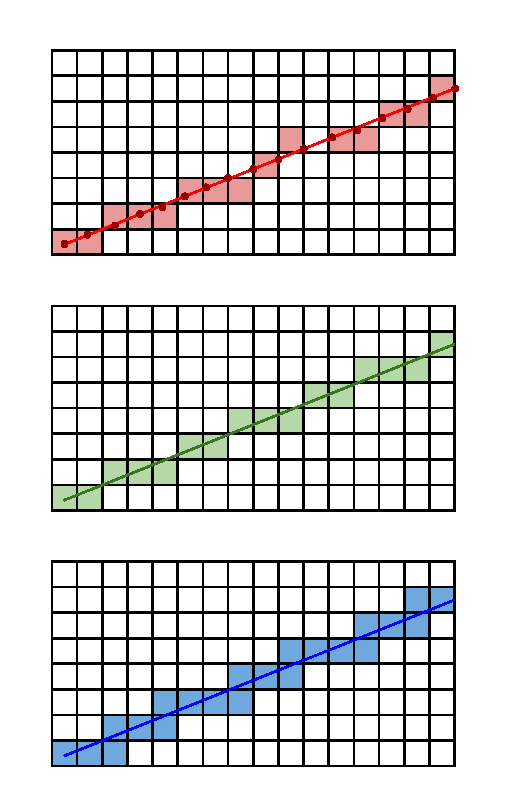
\includegraphics[scale=1.00]{Trace.eps}
\caption{Example of sampling patterns for fixed-step traversal, traversal by standard line raster, and the raster-line traversal used by PolyVox (in red, green, and blue, respectively).}
\end{figure}


To solve these issues, the ray tracer was modified to perform what we have referred to as raster-line tracing, which has ray traces traverse the grid of voxels in a manner similar to how raster-line algorithms draw lines on a rasterized image \cite{rasterline}. There are some slight differences between the program’s raster-line tracing and commonly used raster-line algorithms. Instead of simply traversing the grid such that one element is traversed per column of the trace’s longest dimension, which can cause intersecting elements to be skipped, the raster-line tracer traverses elements in the order that the trace intersects them, expanding outward from that trace’s origin. An example of these traversal methods each being applied to a line is provided in Figure 1.

While calculating which voxel is intersected next by a trace is more expensive to compute than simply stepping that trace in its direction of travel by a constant amount, the reduced number of iterations and samples as a result of this change more than makes up for this discrepancy. Instead of being sampled upwards of 8 or 16 times, each voxel in the path of a trace is sampled precisely once, which leads to faster overall rendering.

After implementing this change, not only was visual fidelity higher, the amount of active blocks that could be present in PolyVox at a given level of detail increased significantly. Prior to this change, there was difficulty with getting any more than a 3x3x3 grid of blocks with 32x32x32 voxels per block above 90 frames per second. Afterwards, PolyVox was capable of rendering and manipulating a 4x4x4 grid of blocks with identical resolution at or above the 90 frames per second mark.

\subsection{Fixing Transparency}

Up until this term, transparency and occlusion was handled linearly, meaning that the amount to which a light ray was occluded by a voxel was calculated based off of how much distance was traversed through that voxel. This, however, is not necessarily accurate to how light is actually occluded when traveling through a volume. In truth, a proportion of light is occluded for each unit of material traversed, creating an exponential decay curve. The transparency algorithm has since then been amended to more accurately represent this falloff in light contribution.

\subsection{Hierarchical Sampling}

For almost all use cases one can expect PolyVox to be subject to, very few have an even distribution of transparent and opaque colors throughout a generated scene. Generally, most shapes that are “interesting” to humans, and hence are the most likely to be reproduced in PolyVox, have detail concentrated in clumps, with many regions of open space. Thus, if the ray tracer can be informed of how open the space in front of a particular trace is, it may be able to step the trace significantly further than that trace normally would.

To apply this approach to PolyVox’s ray tracer, some additional data structures and programs had to be implemented to calculate and encode the similarity of regions in the virtual space. To these ends, another 3D texture of integers was added to blocks in PolyVox. This 3D texture, called the SkipGrid, encodes the local similarity of the voxels in a block

Specifically, after each brush operation, the SkipGrid is updated such that, for every cube of voxels in the block which have a width
\\~
\\~
\centerline{$ 2n $   where    $ n \in \mathbb{N}_1 $}
\\~
\\~
and are offset from the block’s minor side by
\\~
\\~
\centerline{$v2n$   where   $v \in \mathbb{N}_0 3$}
\\~
\\~
the nth bit of the SkipGrid element located at offset v is set if and only if all voxels in that cube have the same color and surface data.

This allows the ray tracer to skip large swaths of voxels which contain the same information by checking for local similarity in the region of space it is meant to trace through next. This can be done for any level in the hierarchy d and at any trace offset in a block p by reversing the relations above and checking the nth bit of the SkipGrid element at offset vwhere:
\\~
\\~
\centerline{$n = 2d$    and  $v = \lfloor p / 2d \rfloor $}
\begin{figure}[h]
\centering
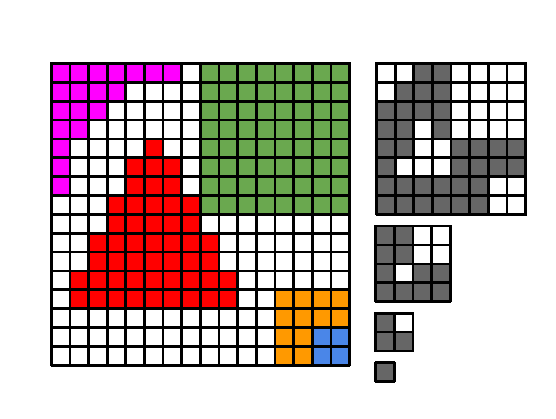
\includegraphics[scale=1.75]{SkipGrid.eps}
\caption{A 2D analog of a ColorGrid/SurfaceGrid (left) and its respective SkipList (right), with the bits of each level of the hierarchy separated and cropped for ease of viewing.}
\end{figure}


By checking bits for a trace’s current position, starting at the highest meaningful level in the hierarchy (the base-2 log of a block’s 3D texture width) and descending to d = 1, the ray tracer, if it finds any set bits, may calculate the result of the trace through the corresponding region as a traversal through one large voxel, making only one color and surface sample operation in the process. To give a more intuitive idea of how a SkipGrid informs trace traversal, Figure 2 above provides an example of how the contents of a block's voxels correspond to the bits of its SkipGrid.

SkipGrids are only half the width of ColorGrid or SurfaceGrid, are made up only of integers, and are sampled from the highest point in the hierarchy downwards, escaping early if any set bits are found. Additionally, when a set bit indicating local similarity is found, the ColorGrid and SurfaceGrid are sampled at the most minor of the voxels in the region of similarity. This structure and behavior means that the cost of the memory fetches made by the ray tracer into the SkipGrid, ColorGrid, and SurfaceGrid during each step are minimized by the density of frequently-used information in memory, keeping the cache hot.

After the addition of this feature, the rendering capacity of PolyVox increased significantly. While, previously, PolyVox could only be used comfortably at block resolutions up to 64 voxels per side, PolyVox can now comfortably render block resolutions up to 128 voxels per side. At resolutions of 32 and 64, PolyVox is also able to increase the relative number of blocks in the space as well, although only up to a number of voxels comparable to standard use with a resolution of 128.

\subsection{Brush Scaling}

\begin{figure}[h]
\centering
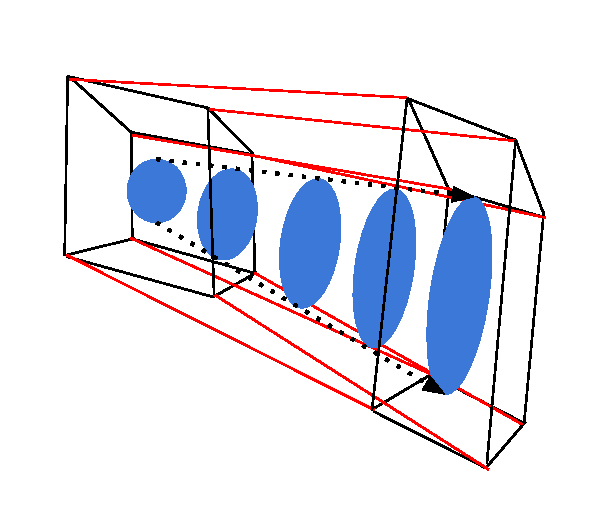
\includegraphics{Transform.eps}
\caption{A diagram portraying how the starting and ending transform of a brush stroke, represented by the left and right boxes, are used to deposit voxels as part of a continuous body, with cross sections of the interpolated brush tip shown in blue.}
\end{figure}


As a matter of basic utility, the team decided that, in addition to controlling the position, color, and opacity of the brush, users should also be able to scale the brush. The ability to modify the scale of the brush tip has always existed in the brush compute shader. This is because the brush relies upon two 4x4 matrices, indicating starting and ending transformation, which includes scale. An example of how these transformations are used to create a brush stroke is provided in Figure 3. Because of this pre-existing capability, the middle end and front end enabled the user to manipulate the scale of the brush tip simply by exposing the scale factors of these transformations via the joystick of the right controller.

\subsection{Canvas Scaling and Transformation}

\begin{figure}[h]
\centering
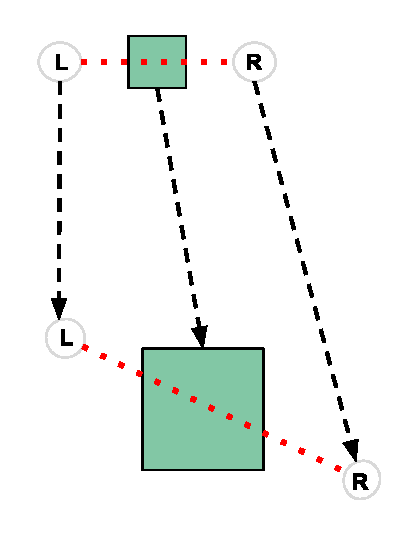
\includegraphics{Scaling.eps}
\caption{A diagram showing how downwards, rightwards, and outwards movement of the left and right controllers causes the scene to correspondingly scale upwards while translating downwards and rightwards.}
\end{figure}


Along the lines of brush scaling, the team also deemed it useful for the user to be able to scale and move the contents of the scene. This was done by taking the positions of the left and right controllers during the current and previous frame, scaling the blocks in the scene by the ratio of the current and previous distances between the left and right controllers, then displacing these blocks such that their distance from the midpoint between the two controllers is equivalently scaled. This means that, when the canvas scaling and moving feature is active, pulling the two controllers apart upscales the scene away from the space in between the controllers and, likewise, pulling the two controllers together downscales the scene towards the space in between the controllers. Additionally, this operation translates the contents of the scene at the same rate and direction of displacement as the midpoint between the controllers. An example of how controller movements can affect the contents of the virtual space is provided in Figure 4.

The inclusion of this feature, overall, has made navigation and inspection of large scenes easier.



\iffalse
\begin{minted}
[
frame=lines,
framesep=2mm,
baselinestretch=1.2,
linenos
]{C}
void CubeBack(int x, int y, int z, int block)
    {
        tempVerts.Add(new Vector3(x, y - 1, z));
        tempVerts.Add(new Vector3(x, y, z));
        tempVerts.Add(new Vector3(x + 1, y, z));
        tempVerts.Add(new Vector3(x + 1, y - 1, z));

        Vector2 color = new Vector2(0, 0);

        if (Block(x, y, z) == 1)
        {
            color = blue;
        }
        else if (Block(x, y, z) == 2)
        {
            color = green;
        }
        else if (Block(x, y, z) == 3)
        {
            color = red;
        }
        else if (Block(x, y, z) == 4)
        {
            color = yellow;
        }

        Cube(color);

    }
\end{minted}
\fi


\section{Conclusion}

Overall, PolyVox now has several new features and several improvements to old ones. In the front end, there are now diegetic interfaces for the manipulation of brush tip color and transparency. Additionally, the front end now offers the ability to change both the scale of the brush tip as well as the scale and position of the canvas. In the middle end, not only have these new features been linked to the operation of the back end, but the preservation of brush scale across saving and loading has been added. Lastly, in the back end, optimizations in storage and processing have enabled PolyVox to represent more complex scenes and render them at faster rates.

In the future, the PolyVox team plans to make three final efforts before the day of expo. The first of these is the inclusion of a brush cursor, which conveys to the user the position, scale, color, and transparency of the voxels deposited by the virtual brush. The second goal the team will push for is to test multiple UI configurations, potentially locking it to different reference frames, such as the head or left controller. Lastly, it is hoped that PolyVox may be rigorously tested for its performance in various situations in order to potentially catch and fix yet unknown bugs before the day of expo.


\end{document}
